\documentclass{article}




\usepackage{fullpage}
%\usepackage{nopageno}
\usepackage{amsmath}
\usepackage{amsfonts}
\usepackage{graphicx}
\usepackage{framed}
\usepackage{algorithmic}
\usepackage{xcolor}

\definecolor{dark_red}{rgb}{0.5,0.0,0.0}
\definecolor{dark_green}{rgb}{0.0,0.5,0.0}
\definecolor{dark_blue}{rgb}{0.0,0.0,0.5}
\definecolor{blue}{rgb}{0.0,0.0,1.0}

\newcommand{\dr}[1]{\textcolor{dark_red}{#1}}
\newcommand{\dg}[1]{\textcolor{dark_green}{#1}}
\newcommand{\db}[1]{\textcolor{dark_blue}{#1}}
\newcommand{\blue}[1]{\textcolor{blue}{#1}}


\title{MATH2860 - 01 Project \#1}
\date{Summer 2021}

\begin{document}

\maketitle

\begin{tabular}{cc}
\parbox{0.5\textwidth}{
This project will involve the analysis of electric circuits such as the circuit depicted on the right. Essential terminology will be defined, and an analysis approach known has {\bf node analysis} will be presented. 
} & \parbox{0.5\textwidth}{
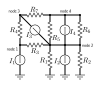
\includegraphics[width = 0.5\textwidth]{complex_circuit_3}
}
\end{tabular}




\section{Terminology}

To describe simple electric circuits, a few basic terms need to be defined:
\begin{itemize}
\item {\bf Voltage}, also referred to as ``electric potential" is in essence ``electrical pressure". When two conductors are at different voltages, electric charge flows from the conductor at a higher electric potential to the conductor at a lower electric potential. Voltage is measured using ``volts" (V), and voltage variables often use the symbol \(V\).
%%%%%%%%%%%%%%%%
\item {\bf Current} is the rate at which electric charge passes a specified boundary, often a circuit component. The passage of negative charge backwards is indistinguishable from the passage of positive charge forwards. When current is measured in the opposite direction, its sign is reversed. Current is measured using ``Amperes" (A). Amperes also measure the rate of charge accumulation at a specific point. Current variables often use the symbol \(I\).
\end{itemize}

\begin{tabular}{cc}
\parbox{0.5\textwidth}{ 
\begin{itemize}
\item In an electric circuit, a {\bf node} is a continuous uninterrupted span of conducting material. Any two points in the circuit that can be connected by a path that does not pass through any circuit components or empty space are part of the same node, an example of which is depicted on the right. On the right, the branching wires that connect the visible components form a single node. The most important detail regarding nodes is that all points on the node have the same voltage. In circuit analysis, nodes are treated as single points connected by the various circuit components. 
\end{itemize}
} & \parbox{0.5\textwidth}{
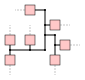
\includegraphics[width = 0.5\textwidth]{circuit_node_definition}
}
\end{tabular}

%\begin{itemize}
%\item At a specific node, the {\bf current flux} is the rate at which the node is accumulating or losing charge. The ``outwards flux" is the rate at which the node is losing charge, and the ``inwards flux", which is the negative of the outwards flux, is the rate at which the node is accumulating electric charge. The outwards flux is the sum of all currents leaving the node, and the inwards flux is the sum of all currents entering the node, and are measured using Amperes. For most nodes, the total flux is \(0\text{A}\) since any charge that enters a node must also leave it. Flux variables often use the symbol \(\Phi\). 
%\end{itemize}

\begin{tabular}{cc}
\parbox{0.75\textwidth}{
\begin{itemize}
\item The {\bf ground node} is a node whose voltage is set to \(0\text{V}\). The voltage of all nodes is measured ``relative" to the ground node. The ground node is not explicitly depicted in circuit diagrams, but an electrical connection to the ground node is denoted by the symbol on the right.
\end{itemize}
} & \parbox{0.25\textwidth}{
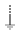
\includegraphics[width = 0.15\textwidth]{ground}
}
\end{tabular}

\begin{itemize}
\item A {\bf circuit component} is an object that connects \(2\) or more nodes in an electric circuit. In this project, the only components that will be used are ``current sources" and ``resistors". 
\item A {\bf current source} transfers a fixed current of \(I\) from a source node to a destination node. %The inwards current flux of the source/starting node \(\Phi_{\text{start}}\) is reduced by \(I\), while the inwards current flux of the destination/ending node \(\Phi_{\text{end}}\) is increased by \(I\).

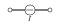
\includegraphics[width = 0.6\textwidth]{current_source}
%%%%%%%%%%%%%%%%
\item A {\bf resistor} is a circuit component that connects two nodes, and the current that flows from the high voltage node to the low voltage node is proportional to the voltage difference between the two nodes.

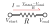
\includegraphics[width = 0.6\textwidth]{resistor} 

The {\bf resistance} \(R\) is the voltage required to propel each ampere of current through the resistor. The voltage difference required to propel a current of \(I\) is:
\[V_{\text{start}} - V_{\text{end}} = R I\] 
Resistance is measured using ``Ohms" (\(\Omega\)). \(1\Omega\) is \(1\text{V}\) per \(1\text{A}\).

The symbol \(G\) will often be used to denote the reciprocal of the resistance, referred to as the ``conductivity": \(G = 1/R\).
\end{itemize}



\section{Setting up the linear system}

Given a circuit diagram with all current sources and resistances known, the goal of {\bf node analysis} is to compute the voltage at each of the non-ground nodes. Let \(n\) denote the number of non-ground nodes, and index the non-ground nodes from \(1\) to \(n\). Let \(V_1\), \(V_2\), ..., \(V_n\) denote the voltages at each of the non-ground nodes. All charge that enters a node must also leave it, and the total current that is leaving or entering a node must be \(0\). This current can be divided into two parts: the current that is entering the node as a result of the current sources, and the current that is draining from the node via the resistors. The rate at which current is pumped into node \(i\) by the current sources is equal to the rate at which current is draining through the resistors, and this common value will be denoted via \(\Phi_i\). The value of \(\Phi_i\) can be computed directly from the circuit diagram by identifying the current sources that are connected to node \(i\). The current sources that pump into node \(i\) add to \(\Phi_i\), while the current sources that drain from node \(i\) subtract from \(\Phi_i\). In the image below,
\[\Phi_i = (I_{\text{in},1} + I_{\text{in},2} + ... + I_{\text{in},k_{\text{in}}}) - (I_{\text{out},1} + I_{\text{out},2} + ... + I_{\text{out},k_{\text{out}}})\]

The rate at which current drains through the resistors is determined by the node voltages. Each connected resistor adds to the total current that is draining through the resistors. The current that drains through a resistor \(R_g\) that connects node \(i\) to the ground node is \(\frac{V_i - 0}{R_g} = \frac{V_i}{R_g}\). The current that drains through a resistor \(R_n\) that connects node \(i\) to another node \(j\) is \(\frac{V_i - V_j}{R_n}\). In the image below, the total current drain through the resistors is:
\begin{align*}
\Phi_i = & \left(\frac{V_i}{R_{g,1}} + \frac{V_i}{R_{g,2}} + ... + \frac{V_i}{R_{g, k_g}}\right) + \left(\frac{V_i - V_{j,1}}{R_{n,1}} + \frac{V_i - V_{j,2}}{R_{n,2}} + ... + \frac{V_i - V_{j,k_n}}{R_{n, k_n}}\right) \\
= & \left((\frac{1}{R_{g,1}} + \frac{1}{R_{g,2}} + ... + \frac{1}{R_{g,k_g}}) + (\frac{1}{R_{n,1}} + \frac{1}{R_{n,2}} + ... + \frac{1}{R_{n,k_n}})\right)V_i - \frac{V_{j,1}}{R_{n,1}} - \frac{V_{j,2}}{R_{n,2}} - ... - \frac{V_{j,k_n}}{R_{n,k_n}}
\end{align*}

By equating the two different expressions for \(\Phi_i\), a linear equation associated with node \(i\) is formed. The value of \(\Phi_i\) computed from the current sources is the constant, and the expression for \(\Phi_i\) above computed from the resistances gives the coefficients of the voltages \(V_1\), \(V_2\), ..., \(V_n\). 

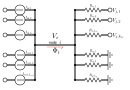
\includegraphics[width = \textwidth]{current_flux}

Similar to how there is an unknown voltage \(V_i\) associated with each non-ground node \(i\), there is an equation associated associated with each non-ground node \(i\) centered around the common value of \(\Phi_i\). In summary, the linear system in matrix vector form is:
\[\begin{bmatrix}
a_{1,1} & a_{1,2} & \cdots & a_{1,n} \\ 
a_{2,1} & a_{2,2} & \cdots & a_{2,n} \\ 
\vdots & \vdots & \ddots & \vdots \\
a_{n,1} & a_{n,2} & \cdots & a_{n,n} 
\end{bmatrix}\begin{bmatrix}
V_1 \\ V_2 \\ \vdots \\ V_n 
\end{bmatrix} = \begin{bmatrix}
\Phi_1 \\ 
\Phi_2 \\ 
\vdots \\ 
\Phi_n 
\end{bmatrix}\]

To derive the constant vector \(\begin{bmatrix} \Phi_1 \\ \Phi_2 \\ \vdots \\ \Phi_n \end{bmatrix}\), each of the current sources need to be examined in sequence. Start by initializing \(\Phi_i = 0\) for each non-ground node \(i\). For each current source, do the following: Let \(I\) denote the current being pumped by the current source under consideration.
\begin{itemize}
\item If the starting node is not a ground-node, and has an index of \(i\), then {\bf subtract} \(I\) from \(\Phi_i\). 
\item If the ending node is not a ground-node, and has an index of \(i\), then {\bf add} \(I\) to \(\Phi_i\). 
\end{itemize}

To derive the coefficient matrix, \(A = \begin{bmatrix}
a_{1,1} & a_{1,2} & \cdots & a_{1,n} \\ 
a_{2,1} & a_{2,2} & \cdots & a_{2,n} \\ 
\vdots & \vdots & \ddots & \vdots \\
a_{n,1} & a_{n,2} & \cdots & a_{n,n} 
\end{bmatrix}\), each of the resistors need to be examined in sequence. Start by initializing \(a_{i,j} = 0\) for each pair of non-ground nodes \(i\) and \(j\). For each resistor, do the following: Let \(R\) denote the resistance of the current resistor.
\begin{itemize}
\item If both terminals of the resistor are not the ground-node, and have indices of \(i\) and \(j\), then {\bf add} \(1/R\) to both \(a_{i, i}\) and \(a_{j, j}\), and {\bf subtract} \(1/R\) from both \(a_{i,j}\) and \(a_{j,i}\). 
\item If one of the terminals is the ground node, let \(i\) denote the index of the non-ground node. {\bf Add} \(1/R\) to \(a_{i,i}\). 
\item If both terminals are the ground node, then ignore the resistor.
\end{itemize}

To better explain the process of computing the constant vector and coefficient matrix, the following examples will be given:


\section{Example circuits}

%%%%%%%%%%%%%%%%% SIMPLEST CIRCUIT 
\subsection{The simplest circuit}

\begin{tabular}{cc}
\parbox{0.5\textwidth}{
This is the simplest possible circuit.

Let \(G_1 = 1/R_1\). 

There is only \(1\) non-ground node, so the only unknown is \(V_1\). 

The single current source delivers a current of \(I_1\) to node \(1\), so \(\Phi_1 = I_1\). 

The single resistor contributes \(G_1 = 1/R_1\) to \(a_{1,1}\), the only entry of \(A\). 

The matrix vector system is:
\[\begin{bmatrix} G_1 \end{bmatrix}\begin{bmatrix} V_1 \end{bmatrix} = \begin{bmatrix} I_1 \end{bmatrix}\]
} & \parbox{0.5\textwidth}{
\includegraphics[width = 0.5\textwidth]{simplest_circuit}
}
\end{tabular}



%%%%%%%%%%%%%%%%% SIMPLEST CIRCUIT 2
\subsection{A 1 node parallel circuit}

\begin{tabular}{cc}
\parbox{0.5\textwidth}{
Let \(G_1 = 1/R_1\) and \(G_2 = 1/R_2\). 

There is only \(1\) non-ground node, so the only unknown is \(V_1\). 

The single current source delivers a current of \(\Phi_1 = I_1\) to node \(1\). 

Resistor \(R_1\) contributes \(G_1\) to \(a_{1,1}\), and resistor \(R_2\) contributes \(G_2\) to \(a_{1,1}\).

The matrix vector system is:  
\[\begin{bmatrix} G_1 + G_2 \end{bmatrix}\begin{bmatrix} V_1 \end{bmatrix} = \begin{bmatrix} I_1 \end{bmatrix}\]
} & \parbox{0.5\textwidth}{
\includegraphics[width = 0.5\textwidth]{simplest_circuit_2}
}
\end{tabular}



%%%%%%%%%%%%%%%%% SERIES CIRCUIT 1 
\subsection{A 2 node series circuit}

\begin{tabular}{cc}
\parbox{0.5\textwidth}{
Let \(G_1 = 1/R_1\) and \(G_2 = 1/R_2\). 

There are \(2\) non-ground nodes, so the unknowns are \(V_1\) and \(V_2\). 

The single current source delivers a current of \(\Phi_2 = I_1\) to node \(2\), while \(\Phi_1\) remains at \(0\). 

\begin{itemize}
\item Resistor \(R_1\) contributes \(G_1\) to \(a_{1,1}\). 
\item Resistor \(R_2\) contributes \(G_2\) to \(a_{1,1}\) and \(a_{2,2}\), and subtracts \(G_2\) from \(a_{1,2}\) and \(a_{2,1}\).
\end{itemize}

The matrix vector system is: 
\[\begin{bmatrix} G_1 + G_2 & -G_2 \\ -G_2 & G_2 \end{bmatrix}
\begin{bmatrix} V_1 \\ V_2 \end{bmatrix} = 
\begin{bmatrix} 0 \\ I_1 \end{bmatrix}\]
} & \parbox{0.5\textwidth}{
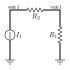
\includegraphics[width = 0.5\textwidth]{series_circuit_1}
}
\end{tabular}



%%%%%%%%%%%%%%%%% SERIES CIRCUIT 2 
\subsection{A 3 node circuit}

\begin{tabular}{cc}
\parbox{0.5\textwidth}{  
Let \(G_1 = 1/R_1\), \(G_2 = 1/R_2\), and \(G_3 = 1/R_3\).      

There are \(3\) non-ground nodes, so the unknowns are \(V_1\), \(V_2\), and \(V_3\). 

The current sources deliver a current of \(\Phi_1 = -I_1\) to node \(1\), and a current of \(\Phi_3 = I_2\) to node \(3\), while \(\Phi_2\) remains at \(0\).

\begin{itemize}
\item The resistor that connects node \(1\) to the ground contributes \(G_1\) to \(a_{1,1}\). 
\item The resistor that links nodes \(1\) and \(2\) contributes \(G_2\) to \(a_{1,1}\) and \(a_{2,2}\), and subtracts \(G_2\) from \(a_{1,2}\) and \(a_{2,1}\). 
\item The resistor that links nodes \(2\) and \(3\) contributes \(G_3\) to \(a_{2,2}\) and \(a_{3,3}\), and subtracts \(G_3\) from \(a_{2,3}\) and \(a_{3,2}\).
\end{itemize}

The matrix vector system is:
\[\begin{bmatrix} G_1 + G_2 & -G_2 & 0 \\ -G_2 & G_2 + G_3 & -G_3 \\ 0 & -G_3 & G_3\end{bmatrix}
\begin{bmatrix} V_1 \\ V_2 \\ V_3 \end{bmatrix} = 
\begin{bmatrix} -I_1 \\ 0 \\ I_2 \end{bmatrix}\]
} & \parbox{0.5\textwidth}{
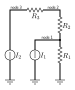
\includegraphics[width = 0.5\textwidth]{series_circuit_2}
}
\end{tabular}



%%%%%%%%%%%%%%%%% COMPLEX CIRCUIT 1 
\subsection{A circuit with multiply linked nodes}

\parbox{0.7\textwidth}{
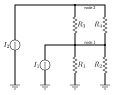
\includegraphics[width = 0.7\textwidth]{complex_circuit_1}
}

Let \(G_1 = 1/R_1\), \(G_2 = 1/R_2\), \(G_3 = 1/R_3\), and \(G_4 = 1/R_4\).                 

There are \(4\) non-ground nodes, so the unknowns are \(V_1\), \(V_2\), \(V_3\), and \(V_4\). 

The current sources deliver a current of \(\Phi_1 = I_1\) to node \(1\), and deliver a current of \(\Phi_2 = I_2\) to node \(2\).

\begin{itemize} 
\item The resistors that connect node \(1\) to the ground contribute \(G_1 + G_2\) to \(a_{1,1}\). 
\item The resistors that link nodes \(1\) and \(2\) contribute \(G_3 + G_4\) to \(a_{1,1}\) and \(a_{2,2}\), and subtract \(G_3 + G_4\) from \(a_{1,2}\) and \(a_{2,1}\). 
\end{itemize}

The matrix vector system is:
\[\begin{bmatrix} G_1 + G_2 + G_3 + G_4 & -G_3 - G_4 \\ -G_3 - G_4 & G_3 + G_4 \end{bmatrix}
\begin{bmatrix} V_1 \\ V_2 \end{bmatrix} = 
\begin{bmatrix} I_1 \\ I_2 \end{bmatrix}\]




%%%%%%%%%%%%%%%%% COMPLEX CIRCUIT 2 
\subsection{A circuit with a bridge}

\parbox{0.7\textwidth}{
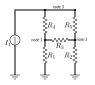
\includegraphics[width = 0.7\textwidth]{complex_circuit_2}
}

Let \(G_1 = 1/R_1\), \(G_2 = 1/R_2\), \(G_3 = 1/R_3\), \(G_4 = 1/R_4\), and \(G_5 = 1/R_5\).            

There are \(3\) non-ground nodes, so the unknowns are \(V_1\), \(V_2\), and \(V_3\). 

The current sources deliver a current of \(\Phi_3 = I_1\) to node \(3\), while \(\Phi_1\) and \(\Phi_2\) remain at \(0\).

\begin{itemize}
\item The resistor that connects node \(1\) to the ground contributes \(G_1\) to \(a_{1,1}\). 
\item The resistor that connects node \(2\) to the ground contributes \(G_2\) to \(a_{2,2}\). 
\item The resistor that links nodes \(1\) and \(2\) contributes \(G_3\) to \(a_{1,1}\) and \(a_{2,2}\), and subtracts \(G_3\) from \(a_{1,2}\) and \(a_{2,1}\). 
\item The resistor that links nodes \(1\) and \(3\) contributes \(G_4\) to \(a_{1,1}\) and \(a_{3,3}\), and subtracts \(G_4\) from \(a_{1,3}\) and \(a_{3,1}\). 
\item The resistor that links nodes \(2\) and \(3\) contributes \(G_5\) to \(a_{2,2}\) and \(a_{3,3}\), and subtracts \(G_5\) from \(a_{2,3}\) and \(a_{3,2}\).    
\end{itemize}

The matrix vector system is:
\[\begin{bmatrix} G_1 + G_3 + G_4 & -G_3 & -G_4 \\ -G_3 & G_2 + G_3 + G_5 & -G_5 \\ -G_4 & -G_5 & G_4 + G_5 \end{bmatrix}
\begin{bmatrix} V_1 \\ V_2 \\ V_3 \end{bmatrix} = 
\begin{bmatrix} 0 \\ 0 \\ I_1 \end{bmatrix}\]



%%%%%%%%%%%%%%%%% COMPLEX CIRCUIT 3 
\subsection{A complex circuit}


\parbox{0.75\textwidth}{
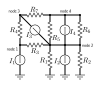
\includegraphics[width = 0.75\textwidth]{complex_circuit_3}
} 

Let \(G_1 = 1/R_1\), \(G_2 = 1/R_2\), \(G_3 = 1/R_3\), \(G_4 = 1/R_4\), \(G_5 = 1/R_5\), \(G_6 = 1/R_6\), and \(G_7 = 1/R_7\).           

There are \(4\) non-ground nodes, so the unknowns are \(V_1\), \(V_2\), \(V_3\), and \(V_4\). 

The current sources delivers a total current of \(\Phi_1 = -I_1\) to node \(1\), a total current of \(\Phi_2 = - I_2 - I_3 - I_4\) to node \(2\), a total current of \(\Phi_3 = I_3\) to node \(3\), and a total current of \(\Phi_4 = I_4\) to node \(4\).

\begin{itemize}
\item The resistors that connect node \(2\) to the ground contribute \(G_1 + G_2\) to \(a_{2,2}\). 
\item The resistor that connects nodes \(1\) and \(2\) contributes \(G_3\) to \(a_{1,1}\) and \(a_{2,2}\), and subtracts \(G_3\) from \(a_{1,2}\) and \(a_{2,1}\). 
\item The resistor that connects nodes \(1\) and \(3\) contributes \(G_4\) to \(a_{1,1}\) and \(a_{3,3}\), and subtracts \(G_4\) from \(a_{1,3}\) and \(a_{3,1}\). 
\item The resistors that connect nodes \(2\) and \(4\) contribute \(G_5 + G_6\) to \(a_{2,2}\) and \(a_{4,4}\), and subtract \(G_5 + G_6\) from \(a_{2,4}\) and \(a_{4,2}\). 
\item The resistor that connects nodes \(3\) and \(4\) contributes \(G_7\) to \(a_{3,3}\) and \(a_{4,4}\), and subtracts \(G_7\) from \(a_{3,4}\) and \(a_{4,3}\). 
\end{itemize}

The matrix vector system is:
\[\begin{bmatrix} 
G_3 + G_4 & -G_3 & -G_4 & 0 \\ 
-G_3 & G_1 + G_2 + G_3 + G_5 + G_6 & 0 & -G_5 - G_6 \\ 
-G_4 & 0 & G_4 + G_7 & -G_7 \\ 
0 & -G_5 - G_6 & -G_7 & G_5 + G_6 + G_7  
\end{bmatrix}
\begin{bmatrix} V_1 \\ V_2 \\ V_3 \\ V_4 \end{bmatrix} = 
\begin{bmatrix} -I_1 \\ -I_2 - I_3 - I_4 \\ I_3 \\ I_4 \end{bmatrix}\]




%%%%%%%%%%%%%%%%% COMPLEX CIRCUIT 4 
\subsection{A $2^{\text{nd}}$ complex circuit}

\parbox{0.7\textwidth}{
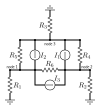
\includegraphics[width = 0.7\textwidth]{complex_circuit_4}
} 

Let \(G_1 = 1/R_1\), \(G_2 = 1/R_2\), \(G_3 = 1/R_3\), \(G_4 = 1/R_4\), \(G_5 = 1/R_5\), and \(G_6 = 1/R_6\)    

There are \(3\) non-ground nodes, so the unknowns are \(V_1\), \(V_2\), and \(V_3\). 

The current sources delivers a total current of \(\Phi_1 = I_2 - I_3\) to node \(1\), a total current of \(\Phi_2 = I_3 - I_1\) to node \(2\), a and total current of \(\Phi_3 = I_1 - I_2\) to node \(3\).

\begin{itemize}
\item The resistor that connects node \(1\) to the ground contributes \(G_1\) to \(a_{1,1}\). 
\item The resistor that connects node \(2\) to the ground contributes \(G_2\) to \(a_{2,2}\). 
\item The resistor that connects node \(3\) to the ground contributes \(G_3\) to \(a_{3,3}\). 
\item The resistor that connects nodes \(2\) and \(3\) contributes \(G_4\) to \(a_{2,2}\) and \(a_{3,3}\), and subtracts \(G_4\) from \(a_{2,3}\) and \(a_{3,2}\). 
\item The resistor that connects nodes \(1\) and \(3\) contributes \(G_5\) to \(a_{1,1}\) and \(a_{3,3}\), and subtracts \(G_5\) from \(a_{1,3}\) and \(a_{3,1}\). 
\item The resistor that connects nodes \(1\) and \(2\) contributes \(G_6\) to \(a_{1,1}\) and \(a_{2,2}\), and subtracts \(G_6\) from \(a_{1,2}\) and \(a_{2,1}\). 
\end{itemize}

The matrix vector system is:        
\[\begin{bmatrix} 
G_1 + G_5 + G_6 & -G_6 & -G_5 \\ 
-G_6 & G_2 + G_4 + G_6 & -G_4 \\ 
-G_5 & -G_4 & G_3 + G_4 + G_5 
\end{bmatrix}
\begin{bmatrix} V_1 \\ V_2 \\ V_3 \end{bmatrix} = 
\begin{bmatrix} I_2 - I_3 \\ I_3 - I_1 \\ I_1 - I_2 \end{bmatrix}\]




\section{Assignment}

You are provided with an incomplete Matlab file. You must complete the Matlab file so that the file can be used for the following nodal analysis. The following is a description of the input variables used in the Matlab file:

\begin{itemize}
\item \texttt{num\_of\_nodes} is the number of nodes \(n\) in the circuit. The nodes are hence indexed from \(1\) to \(n\).
\item \texttt{num\_of\_current\_sources} is the number \(k_I\) of current sources.  
\item \texttt{current\_source\_end\_nodes} is an \(k_I \times 2\) array where for each \(i = 1, 2, ..., k_I\), entry \((i, 1)\) stores the node index of the start of current source \(i\), and entry \((i, 2)\) stores the node index of the end of current source \(i\). The ground node is indexed by \(0\).   
\item \texttt{current\_source\_values} is an \(k_I \times 1\) array where for each \(i = 1, 2, ..., k_I\), entry \((i, 1)\) stores the current being pumped by current source \(i\).    
\item \texttt{num\_of\_resistors} is the number \(k_R\) of resistors.  
\item \texttt{resistor\_end\_nodes} is an \(k_R \times 2\) array where for each \(i = 1, 2, ..., k_R\), entries \((i, 1)\) and \((i, 2)\) store the node indices of the terminals of resistor \(i\). The ground node is indexed by \(0\).    
\item \texttt{resistor\_values} is an \(k_R \times 1\) array where for each \(i = 1, 2, ..., k_R\), entry \((i, 1)\) stores the resistance of resistor \(i\).  
\end{itemize} 

{\bf Everywhere \texttt{???} appears you must complete the code.}

{\bf In the circuit below}, there are \(6\) nodes. Using Matlab compute the following. {\bf Submit your Matlab script.} Your Matlab script must compute the asked for values.
\begin{itemize}
\item \(\Phi_i\) at each node. %, the vector:
%\(\begin{bmatrix} \Phi_1 \\ \Phi_2 \\ \Phi_3 \\ \Phi_4 \\ \Phi_5 \\ \Phi_6 \end{bmatrix}\)
\item The \(6 \times 6\) coefficient matrix \(A\)
\item Solve the system 
\(A\begin{bmatrix} V_1 \\ V_2 \\ V_3 \\ V_4 \\ V_5 \\ V_6 \end{bmatrix} = \begin{bmatrix} \Phi_1 \\ \Phi_2 \\ \Phi_3 \\ \Phi_4 \\ \Phi_5 \\ \Phi_6 \end{bmatrix}\)
for the voltage at each node. %, the vector: 
%\(\begin{bmatrix} V_1 \\ V_2 \\ V_3 \\ V_4 \\ V_5 \\ V_6 \end{bmatrix}\)
\end{itemize} 
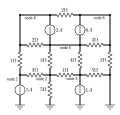
\includegraphics[width = \textwidth]{problem_circuit_1}


\end{document}












